\documentclass[10pt,twocolumn]{article}

% use the oxycomps style file
\usepackage{oxycomps}

% usage: \fixme[comments describing issue]{text to be fixed}
% define \fixme as not doing anything special
\newcommand{\fixme}[2][]{#2}
% overwrite it so it shows up as red
\renewcommand{\fixme}[2][]{\textcolor{red}{#2}}
% overwrite it again so related text shows as footnotes
%\renewcommand{\fixme}[2][]{\textcolor{red}{#2\footnote{#1}}}

% read references.bib for the bibtex data
\bibliography{references}

% include metadata in the generated pdf file
\pdfinfo{
    /Title Git Tutorial for Version Control
    /Author (Julia Chun)
}

% set the title and author information
\title{Git Tutorial for Version Control}
\author{Julia Chun}
\affiliation{Occidental College}
\email{jchun2@oxy.edu}

\begin{document}

\maketitle

\section{Introduction}

This document serves as a tutorial for beginners who are new to version control and git. In this tutorial, basic commands of Git are covered such as in-iting/cloning, adding, committing, and pushing. In addition, stashing, branching and merging will also be discussed. Rather than providing understanding oriented and information oriented content, this tutorial provides learning and problem oriented content that steps through essential concepts and methods needed to effectively utilize Git.  

\section{Git, Github, and GitBash}
For Computer Science students, there is often the need to collaborate on projects where multiple developers could work in parallel. Git is  version control system used by developers to manage and collaborate efficiently on projects. This system allows changes in source code to be tracked during code development and ensures there are no code conflicts between developers. In this tutorial, we will utilize a command-line interface (CLI) called GitBash for Windows systems. This interface allows you to communicate with Git using various commands. We will also utilize a web-based platform called GitHub which allows users to store their code remotely and access it through the network. This platform also allows for effective collaboration and management between developers where code could be manage, shared and tracked. 
\section {Setting up GitBash and Creating a Github repository}
To start 


\section {Basic Commands of Git}
Git/GitBash provides powerful commands to manage version control and collaboration on projects. Some basic commands that are fundamental for the use of effective version control usages are init, clone, commit, push, and pull. Understanding these commands will allow efficient management of projects and effective work in repositories. 

\subsection{Creating a Remote Repository on Github}
To create a repository on Github, navigate to Github.com and login or create an account if you have not done so. If you are not already on the home page of the website, navigate to the home page by clicking the upper-left most icon and clicking the home button. Once on the home page, in the upper-right corner of the page, select the icon with a cross and down-bar and select 'New repository'. \ref{Figure 9}. Once directed to the page, 'Create a new repository', enter the information for your repository such as the repository name, description. Additionally, select whether to make your repository public or private and select the 'Add a README file' button if you would like to create a README file in your repository. A README file could help people understand the purpose of your project. Hence, it is recommended to select this option and write helpful information. 


\subsection{Init/Cloning}
The 'git init' command initializes a new repository on your local machine by creating a new .git sub-directory in your current working directory. 
To start, navigate to your project directory in GitBash to initialize a new Git repository. This could be done by opening your File Explorer and creating a new folder. Then, right click on your create folder and select the option 'open with GitBash'. To initialize a new Git repository in the current directory, type 'git init' on the command line.\ref{Figure 1}. This will create hidden directory named '.git' which stores all the necessary files and metadata for version control. After initializing your repository on GitBash, you may check the status of your repository by using the command 'git status' on the next line.\ref{Figure 2}  Notice that the file name is shown in red text. This indicates that the file is an untracked file, which is a file that have been created within your repository's working directory but have not yet added to the repository's tracking index using the git add command. The file name will be presented in green text when it becomes a tracked file. 


Cloning a repository in Git allows a local copy of a remote repository to be made. This will allow a duplicate of the entire project history from to be made on a local machine and allows changes to be made without affecting the original remote repository. 
To clone a repository, the URL of the remote repository you want to clone must be located. This could be found on the main page of the repository you would like to clone. On GitHub.com, locate and click the green '<>Code button' and under the tab 'Local', copy the URL.\ref{Figure 3} The URL could be copied in three types: HTTP, SSH, and GitHub CLI.  Open Git Bash and change the current working directory to the desired location. This could be done by opening your File Navigator and right clicking on the file you would like to clone the desired repository into. Choose the option 'Open GitBash here', type "git clone" on the command line, and paste the URL.\ref{Figure 4} To verify that the repository is successfully cloned, navigate to the path your repository was cloned and verify that the cloned repository is present.{Figure 5}

If we wanted to clone a repository already associated with our account, we could click on 'File' and 'Clone Repository'. We select the tab 'GitHub.com' which will show all the repositories that are already forked on your account on GitHub.com so you can then take a copy of that repository onto your local machine.





\subsection{Adding}
Adding changes involves staging modifies files for inclusion in the next commit. "Staging" refers to the process of preparing modifications for a commit. When you make modifications to files in your project, Git allows you to selectively choose which changes you would like to add in the next commit. The add command is used before the execution of the commit command. 

To use the add command to add a specific file, type 'git add<path>' where path is the path of the file. \ref{Figure 6} To add all changes in the current directory, type 'git add .' or to add all changes in the entire repository type 'git add --all'. The status of the added changes may be verified by typing 'git status' where files that are staged and ready to be committed are verified. Notice that the file is now presented in green text, indicating it is now being recognized and actively managed by Git. 

\subsection{Committing}
The git commit  commands allows saving of a project's currently staged changes. To commit a change, type "git commit -m". Then, in quotations following the command, type a message describing the commit or changes you are creating.  \ref{Figure 7}The command 'git log' could be used to view the commit history and verify that the commit was successful. This command will display a list of commits showing details such as the message, author, and date. \ref{Figure 8} 
 


\subsection{Pushing}
Pushing changes sends commits made in your local repository to a remote repository. This will allow collaboration with others while keeping the remote repository updated with local changes. 


After your changes have been added and committed, you  may push them onto the remote repository using the 'git push' command followed my the name of the remote repository and branch that you want to be pushed.\ref{FIgure12} After executing this command, you may be prompted to enter your username and password to your GitHub account.\ref To verify that the changes have been successfully uploaded, check the remote branch on the hosting platform.\ref{Figure13}\ref{Figure14}



\subsection{Pulling}
Pulling changes allows changes to be retrieved or fetched from a remote repository and merged into your local repository. The 'git pull' command pulls latest changes from the remote repository and automatically merged into your current local branch. First, navigate to the cloned repository you are working with and open GitBash by right-clicking on the file and selecting the option 'Open GitBash here'. After making changes to a file on the remote repository (GitHub), commit your changes by selecting the 'Commit changes' button on the upper-right most corner. Enter your commit message and select either the option 'Commit directly to the main branch' or 'Create a new branch for this commit and start a pull request'. A Pull Request notifies others about the changes pushed onto a branch in a repository on GitHub. As the request is opened, it could be discussed and reviewed with collaborators before the changes are merged on the main branch. If the 'pull request' option is selected, you may update the name of the request and record any comments. Then select 'Create pull request'. GitHub will then check for any merge conflicts and it will be ready for review. The owner will then review the request and if approved, the pull request will get merged./ref{Figure11}  Type 'git pull' to fetch and download content from the remote repository. The local repository will immediately be updated to match its content./ref{Figure 10}.  Changes could also be pulled the origin master which pulls changes from the 'master' branch of the remote repository called 'origin' and integrates them into your local HEAD branch. The HEAD is a point which you are currently working on. In Git, 'origin' typically refers to the default remote repository and 'master' is often considered the main branch of a Git repository. This could be done by typing 'git pull origin master' on GitBash.  


\section{Advanced Commands}
As you advance in Git, you may encounter scenarios where a more nuanced approach to version control is required. Advance Git commands such as stashing, branching, and merging could provide functionalities for handling these nuanced demands.  

\subsection {Stashes}
Stashing is a feature which allows changes to be temporarily stored that are not ready to be committed yet. This could be useful when you may need to switch to a different task or branch, but am not ready to commit changes. This allows current changes to be saved while you are able to work on something different. 

Before stashing, ensure your working directory has no uncommitted changes. Then, use 'git stash' command on GitBash. This command may only be used when you have changes to stashed but have not committed. Once your changes are stashed, you may continue working on other tasks. To revisit your stashed changes, type the 'git stash apply' command on GitBash. This command will take the most recently saved stash and overwrite the files in the current working tree.   The command 'git stash apply' will stash the most recent stash and this command followed by typing the index number of a particular stash will reapply changes to the stash of the index. The command 'git stash list' may be used to view the stashes that exist with the index number of that stash. The command 'git stash pop' could be used to apply the changes from the most recent stash to your working directory and remove the stash for the stash stack. To discard stashed changes that are no longer needed, you may remove them using the 'git stash drop' command which will remove the most recent stash from the stash stack. 

\subsection {Branches}
Branches allow you to diverge from the main line of development and work on varying features of the project locally. The main branch in Git, named 'main' represents the primary line of development and usually contains the latest version of the project's code.  Each branch in a Git repository can represent an independent line of development with its own commits. This allows effective organization and management of your project.

To create a new branch, type 'git branch' followed by the name branch. The command 'git checkout' will allow you to switch from working in your working directory to a different branch. To start working on your new branch, type 'git checkout' followed by the branch name. Now you may make changes to this branch, add and commit the changes. After the changes are committed, push the committed changes to the origin and the branch should be visible to the remote repository. However, if you navigate to the master branch, you will notice that the created branch is not visible because the new branch is not merged with the master branch. To do this, type 'git checkout master'. Then type  'git merge' followed by the name of the created branch. The new branch should now be available in the master branch.  To create a new branch from an existing branch (usually the main branch) type 'git checkout -b' and enter the name of the new branch you would like to create.  To delete a branch from your local repository, type '-d git branch' followed by the branch name. To delete the branch from the remote repository, type 'git push origin -- delete' followed by the branch name. 

\subsection {Merging and dealing with Merge Conflicts}
Merging allows integration of changes from one branch into another. This is typically done on a feature branch into the main branch which allows incorporation of changes into the main line of development. 

To merge a branch into another branch, the target branch where changes are to be incorporated must be switched. To merge a feature branch into the main branch, switch to the main branch by typing 'git checkout main' on GitBash. Once on the target branch, type 'git merge' followed by the name of the branch to be merged on GitBash in the format 'git merge <branch-name>.

When conflicts occur when Git is unable to merge changes from different branches, a "merge conflict" occurs.

Git will mark the conflicted sections in the affected files when a merge conflict occurs with the less than, equals, and greater than symbols. If you would like to abort the merge, type the command 'git merge --abort' which will cancel the merge and revert you to the status of your work before the merge.  To resolve the differences between the conflicts you may choose between various options. You may accept the current change,which would only accept the changes in your branch, accept incoming change which would only take the incoming changes, accept both changes which keep merge the changes, or compare changes. You may remove the markers and decide which changes to keep. The 'git add' command should be used to stage the modified files and once the conflicts and resolved and stage, commit the merge. After the conflicts are resolved and the changes are committed, the merged changes may be pushed to the remote repository. 
\section{Conclusion}
Mastering Git for version control is a useful skill for those aiming to collaborate effectively in coding projects and maintain code integrity. Fundamental concepts and commands were covered in this tutorial to aid with navigating version control with Git and utilize platforms such as GitHub. 










\begin{figure}
    \centering
    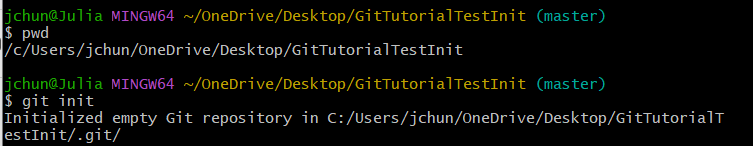
\includegraphics[width=.95\linewidth]{Gitinitnew.png}
    \caption{
        Initializing a repository on GitBash. 
    }
    \label{Figure 1}
\end{figure} 

\begin{figure}
    \centering
    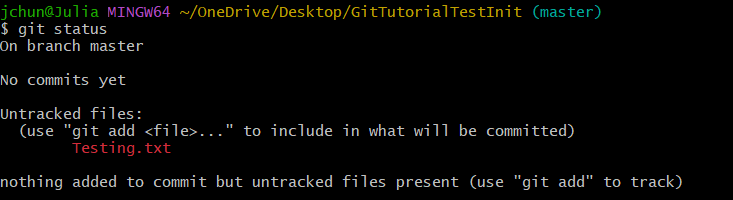
\includegraphics[width=.95\linewidth]{Gitstatus.png}
    \caption{
        Checking the status of the current repository.  
    }
    \label{Figure 2}
\end{figure}
\begin{figure}
    \centering
    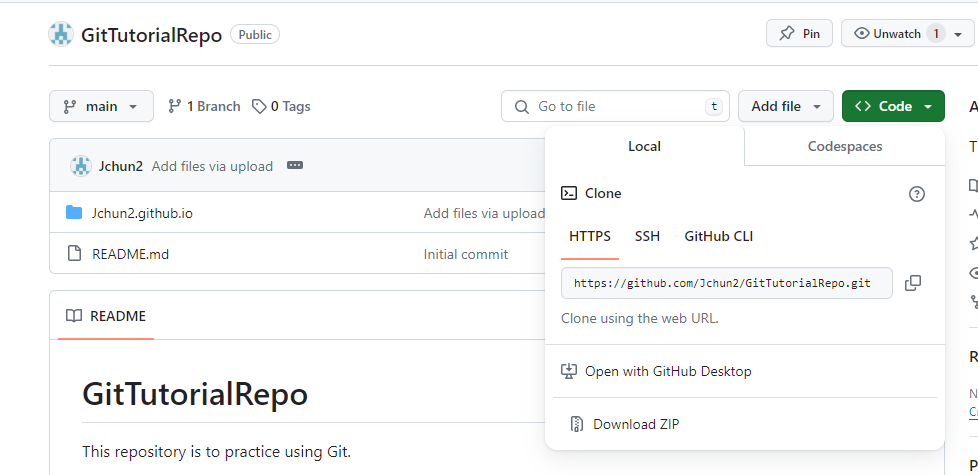
\includegraphics[width=.95\linewidth]{GitCloning.png}
    \caption{
        Copying the URL of the repository to be cloned. 
    }
    \label{Figure 3}
\end{figure}

 

\begin{figure}
    \centering
    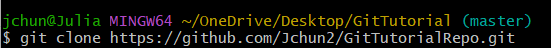
\includegraphics[width=.95\linewidth]{Git CLoinging.png}
    \caption{
        Cloning the repository.  
    }
    \label{Figure 4}
\end{figure}
\begin{figure}
    \centering
    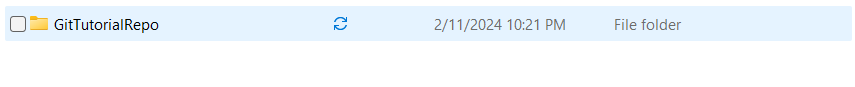
\includegraphics[width=.95\linewidth]{clonedfile.png}
    \caption{
        Verified the cloned repository.  
    }
    \label{Figure 5}
\end{figure}
\begin{figure}
    \centering
    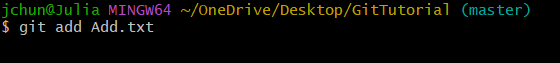
\includegraphics[width=.95\linewidth]{Gitadd.png}
    \caption{
      Using the 'git add' command. 
    }
    \label{Figure 6}
\end{figure}
\begin{figure}
    \centering
    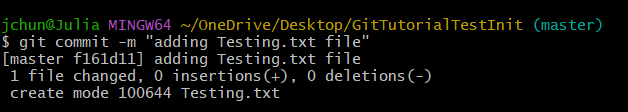
\includegraphics[width=.95\linewidth]{GitcommitaddingTesting.png}
    \caption{
        Committing the adding of the file Testing.txt.   
    }
    \label{Figure 7}
\end{figure}
\begin{figure}
    \centering
    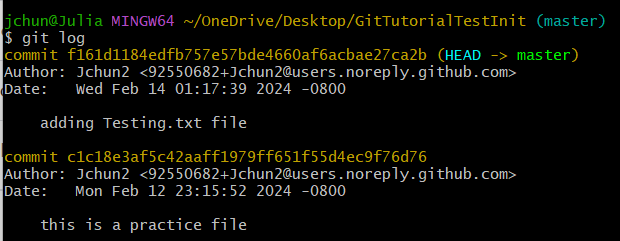
\includegraphics[width=.95\linewidth]{gitlog.png}
    \caption{
        Using the command 'git log'.    
    }
    \label{Figure 8}
\end{figure}
\begin{figure}
    \centering
    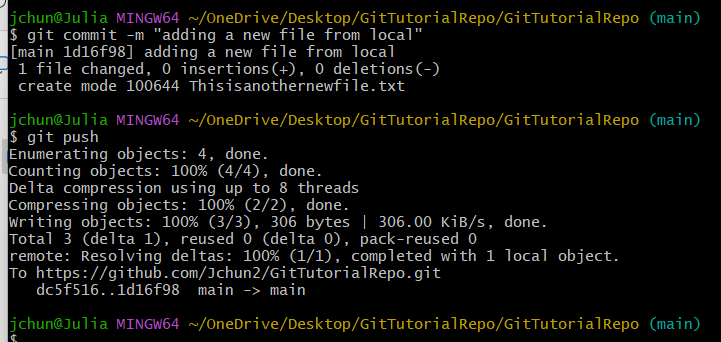
\includegraphics[width=.95\linewidth]{gitpush.png}
    \caption{
        Using the command 'git push'.    
    }
    \label{Figure 12}
\end{figure}
\begin{figure}
    \centering
    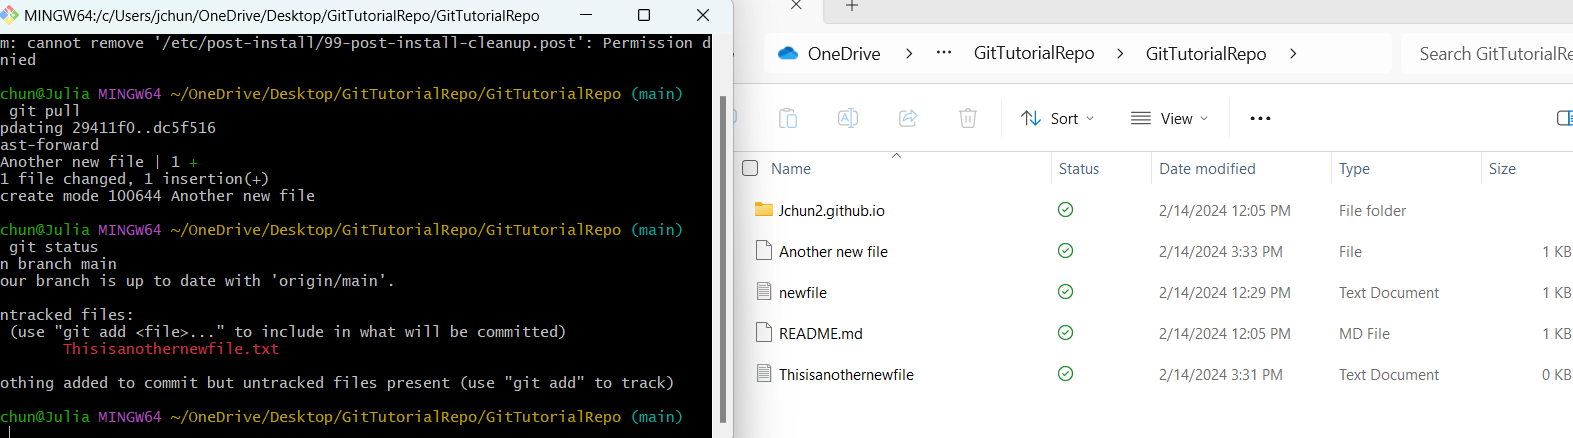
\includegraphics[width=.95\linewidth]{beforepush.png}
    \caption{
        The remote repository before the pushed file.    
    }
    \label{Figure 13}
\end{figure}
\begin{figure}
    \centering
    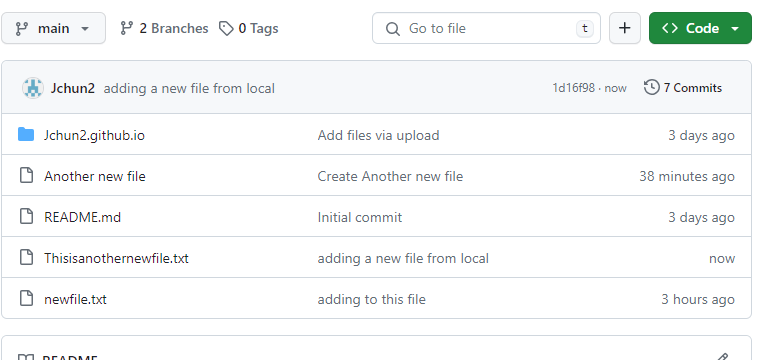
\includegraphics[width=.95\linewidth]{pushaddfille.png}
    \caption{
        The file created from local repository is now present in the remote repository.    
    }
    \label{Figure 14}
\end{figure}
\begin{figure}
    \centering
    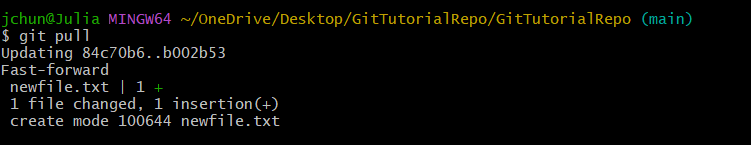
\includegraphics[width=.95\linewidth]{gitpull.png}
    \caption{
        newfile.txt is pulled from the remote repository.   
    }
    \label{Figure 10}
\end{figure}
\begin{figure}
    \centering
    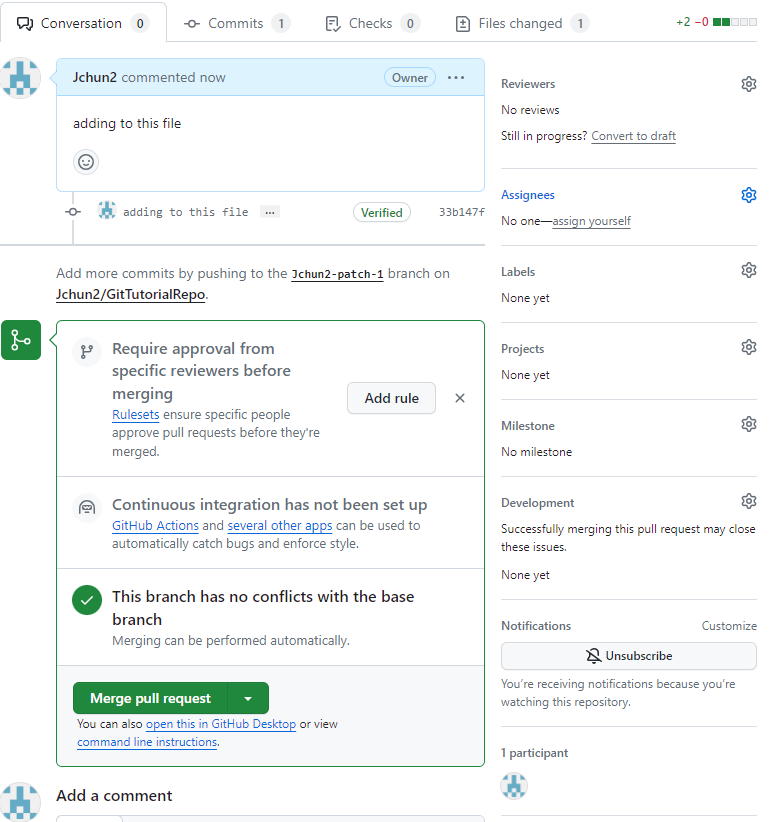
\includegraphics[width=.95\linewidth]{pullrequest.png}
    \caption{
        Creating a pull request.  
    }
    \label{Figure 11}
\end{figure}
\newpage
\newpage
\begin{thebibliography}{100}
\addtolength{\leftmargin}{0.2in} % sets up alignment with the following line.
\setlength{\itemindent}{-0.2in}

\bibitem{website}
{Atlassian. “Git Pull: Atlassian Git Tutorial.” Atlassian, www.atlassian.com/git/tutorials/syncing/git-pull. Accessed 14 Feb. 2024. }
\bibitem{video}
“Git and Github Beginner Tutorial 5 - Branching and Merging.” YouTube, 15 Oct. 2016, youtu.be/GZILYABgAoo?si=l82KkbxdKTwFcTge. 
\bibitem{video}
“Git Branches - Creating and Managing Branches in Git Using Git Branch, Git Merge and Git Checkout.” YouTube, 25 Aug. 2020, youtu.be/oq1FGRTOFBw?si=Iw2HjWPsMw_OxAVW. 
\bibitem{video}
“GITHUB Pull Request, Branching, Merging & Team Workflow.” YouTube, 20 Mar. 2014, youtu.be/oFYyTZwMyAg?si=Tkod87LYnpSjJ-1f. 
\bibitem{website}
“How to Resolve Merge Conflicts in Git.” YouTube, 21 Apr. 2020, youtu.be/xNVM5UxlFSA?si=A6lP5mDKHFx8DusM. 
\bibitem{website}
RefaelRefael                      6, et al. “How Do I Display a Text File Content in CMD?” Stack Overflow, 1 May 1959, stackoverflow.com/questions/17217476/how-do-i-display-a-text-file-content-in-cmd. 
\bibitem{website}
“Using ‘Git Pull Origin Master’ to Download Changes.” Using “Git Pull Origin Master” to Download Changes | Learn Version Control with Git, www.git-tower.com/learn/git/faq/git-pull-origin-master. Accessed 14 Feb. 2024. 
\end{thebibliography}


\printbibliography
\printbibliography

\end{document}
